\section{The Classical Notion of an Autonomous Agent}
\label{sec:classical-agent}

\subsection{Rationality and the perceive-decide-act loop}
\label{subsec:rationality}

A rational agent selects the action that achieves the best outcome or, when outcomes are uncertain, the best expected outcome \cite[Chap.~2]{russellArtificialIntelligenceModern2022}. Such systems are described by the following elements \cite[Chap.~2]{russellArtificialIntelligenceModern2022}:

\begin{itemize}
	\item The \emph{performance measure}, an external criterion that defines the notion of best by scoring the consequences of the agent's behavior on the environment, specified in terms of states of the world.
	\item The \emph{agent function}, the abstract mapping from percepts to actions, where a percept is the perceptual input available to the agent at a given instant.
	\item The \emph{agent program}, the concrete implementation that produces those actions on a physical or computational machine.
\end{itemize}

Figure~\ref{fig:rational-agent} summarizes these elements and their relations.

\begin{figure}[ht]
	\centering
	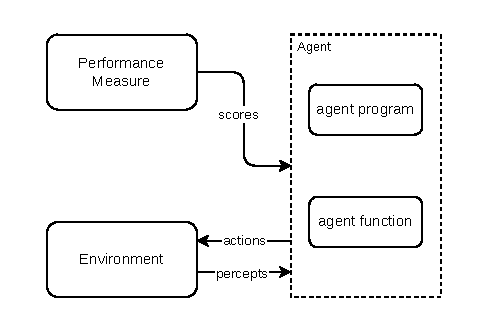
\includegraphics[width=0.6\textwidth]{images/rational_agent.pdf}
	\caption[An autonomous agent]{An autonomous agent}
	\label{fig:rational-agent}
\end{figure}

Independently of its internal design, an agent program implements the same three-step pattern. The system observes the environment, decides what to do, and acts. The action may change the environment; the resulting state is observed, and the cycle repeats. This is the perceive-decide-act loop \cite[Chap.~2]{russellArtificialIntelligenceModern2022}. Rationality is realized in the decide step, where the agent selects the action that, given the available percepts, is expected to maximize the performance measure.

The loop above treats perception as the agent receiving whatever percept the environment provides. Some actions are instead chosen to affect what the agent perceives next rather than to change the state of the environment. This is called information gathering, an action planned for the purpose of reducing the agent's uncertainty about the environment \cite[Chap.~2]{russellArtificialIntelligenceModern2022}. Bajcsy characterizes perception as active, by analogy to biological vision, where the sensing apparatus is continuously adjusted rather than left to record whatever reaches it \cite{bajcsyActivePerception1988}. Under this view, the agent also controls its own data acquisition, through strategies that depend on the goal of the task and on the current state of the interpretation. The choice of what to measure, where to look, and when enough has been observed is formulated as a search that minimizes a loss while seeking the most informative data \cite{bajcsyActivePerception1988}. The control is guided by prior knowledge, in a knowledge-driven regime: the agent's models and expectations direct what it looks for. This has a cost: acquisition can be steered toward what is expected, so unanticipated objects can go undetected \cite{bajcsyActivePerception1988}. The perceive and decide steps are therefore mutually dependent, because the percepts that the decide step acts on are partly the result of earlier choices about what to acquire.

\subsection{Approaches to building agents}
\label{subsec:building-approaches}

Russell and Norvig identify four kinds of agent program that realize the decide step: simple reflex, model-based reflex, goal-based, and utility-based agents \cite[Chap.~2]{russellArtificialIntelligenceModern2022}. Each extends the previous one to remove one of its limitations, and any of the four can in addition be made a learning agent, whose components are acquired from experience instead of being fixed by the designer \cite[Chap.~2]{russellArtificialIntelligenceModern2022}. None of them removes the requirement that the designer specify the task in advance. What changes across the four is the form that the specification takes. Each kind chooses its action from the agent's \emph{current state}, the description of the relevant aspects of the environment at the present instant. A simple reflex agent takes the current state directly from the current percept, but the others reconstruct it from the percept history using a model of the environment \cite[Chap.~2]{russellArtificialIntelligenceModern2022}. Table~\ref{tab:agent-designs} summarizes how each design selects an action, what the designer has to supply, and the limitation that remains.

\begin{itemize}
	\item The \emph{simple reflex agent} realizes the decide step as condition-action rules on the current percept, which works only when the environment is fully observable \cite[Chap.~2]{russellArtificialIntelligenceModern2022}.
	\item The \emph{model-based reflex agent} maintains an internal state to track what the current percept does not reveal, which requires a transition model of how the environment evolves and a sensor model of how its state is reflected in the percepts \cite[Chap.~2]{russellArtificialIntelligenceModern2022}.
	\item The \emph{goal-based agent} adds a description of the desirable situations and selects actions predicted to lead to them, which requires consideration of the future. When a single action does not suffice, this also requires search and planning over a domain model that the designer writes in advance \cite[Chap.~2]{russellArtificialIntelligenceModern2022}. Planning of this kind is computationally costly \cite[Chap.~2]{russellArtificialIntelligenceModern2022}. Hierarchical task network planning reduces the cost by using a plan library of known methods that implement high-level actions, so the planner searches only the sequences allowed by the library instead of the full space of primitive actions \cite[Chap.~11]{russellArtificialIntelligenceModern2022}.
	\item The \emph{utility-based agent} replaces the goal's plain test of whether a state is reached or not with a utility function over states of the world, the internal counterpart of the performance measure, and selects the action that maximizes expected utility \cite[Chap.~2]{russellArtificialIntelligenceModern2022}.
\end{itemize}

Learning is not a separate design for the decide step but a method for improving the components of any of the previous designs \cite[Chap.~2]{russellArtificialIntelligenceModern2022}. A learning agent is decomposed into three components \cite[Chap.~2]{russellArtificialIntelligenceModern2022}. The performance element is the action-selecting program described so far. A learning element modifies it using feedback from a critic, which measures performance against a fixed standard. A problem generator proposes exploratory actions. In its reinforcement-learning instance, the feedback is a reward signal and the agent refines a mapping from percepts to actions through interaction with the environment \cite[Chap.~23]{russellArtificialIntelligenceModern2022}. The cost moves from authoring rules, models, or plans to providing an environment in which to train, a reward function that captures the intended objective, and enough interaction to converge. Dulac-Arnold et al. survey nine challenges that separate laboratory reinforcement learning from production use, including learning from limited samples on the actual system, partial observability and non-stationarity, satisfying safety constraints during training and operation, and specifying a well-posed and aligned reward \cite{dulac-arnoldChallengesRealWorldReinforcement2019}. Each of these typically requires application-specific engineering, and the resulting policy remains tied to the task and to the conditions under which it was trained \cite{dulac-arnoldChallengesRealWorldReinforcement2019}.

\begin{table}[ht]
	\centering
	\small
	\renewcommand{\arraystretch}{1.15}
	\newcolumntype{R}[1]{>{\raggedright\arraybackslash\hsize=#1\hsize}X}
	\begin{tabularx}{\textwidth}{@{}>{\raggedright\arraybackslash}p{2.75cm}R{1.10}R{0.90}R{1.00}@{}}
		\toprule
		Agent type & Action selection & Designer must supply & Principal limitation \\
		\midrule
		Simple reflex & Condition-action rules on the current percept & The rules & Requires a fully observable environment \\
		\addlinespace
		Model-based reflex & Rules over an internal state & Rules, a transition model, a sensor model & No goals and no model of the future \\
		\addlinespace
		Goal-based & Search and planning toward goal states, or refinement from a plan library & A domain model and goals, or a plan library & Planning is costly; competence is bounded by what is authored \\
		\addlinespace
		Utility-based & Maximization of expected utility & A utility function, in addition to a model & The utility function is hard to specify \\
		\addlinespace
		Learning & Any of the above, refined from feedback & A training environment, a reward signal, interaction & The policy is tied to the task and its training conditions \\
		\bottomrule
	\end{tabularx}
	\caption[Comparison of the agent designs]{Comparison of the agent designs.}
	\label{tab:agent-designs}
\end{table}

The decide step is built for a specific task in each of the four designs, whether their components are fixed by the designer or acquired through learning. What the designer must supply is listed in Table~\ref{tab:agent-designs}: the condition-action rules, the transition and sensor models, the domain model and plan library, the utility function, or the training environment and reward signal. Each of these has to be stated in a formal and executable form, over a set of actions fixed in advance, before the agent can act at all.

This requirement is the principal cost of building an agent with these designs. The intended behavior is normally known in informal terms, and the work consists in translating it into a specification that the decide step can execute. This translation demands expertise in the design and in the application domain. It is also incomplete in practice: cases that the specification does not cover produce no useful behavior, and the effort grows with the range of cases that the agent has to handle. The reinforcement-learning case illustrates the same cost in a different form, since the reward signal has to express the intended objective and the training conditions have to reproduce the operating conditions. Each of these requires application-specific engineering \cite{dulac-arnoldChallengesRealWorldReinforcement2019}. Building an agent under these designs is therefore limited less by the loop of Section~\ref{subsec:rationality} than by the difficulty of producing the specification that the decide step needs.
